\documentclass[AL.tex]{subfiles}

\begin{document}


%\hyphenation{equi-va-len-cia}\hyphenation{pro-pie-dad}\hyphenation{res-pec-ti-va-men-te}\hyphenation{sub-es-pa-cio}

\chapter{Complejidad de un problema}

\section{Primeras nociones}
\begin{defi}\
\begin{itemize}
\item Complejidad de un algoritmo $A$: ratio de crecimiento del tiempo de computación del algoritmo, denotado $T_A(n)$
\item Complejidad de un problema $P$: complejidad del ``mejor algoritmo'' (en el sentido de su complejidad) que resuelve $P$. La denotamos $C_P(n)$. 
\end{itemize}
\end{defi}
De la definición se deduce que $C_p(n)\leq T_A(n)$ para $A$ un algoritmo que resuelve $P$.  Si cualquier algoritmo $A$ para resolver $P$ requiere al menos $S_P(n)$, entonces $C_P(n)\geq S_P(n)$. Si $T_A(n)\in\Theta(S_p(n))$, se dice que $C_p(n)=\Theta(T(n))$ y el algoritmo $A$ es \emph{óptimo}. 

\begin{ej}[Matrix-Addition]
El algoritmo más evidente tiene dos bucles (hay un índice para las filas y otro para las columnas), luego $T_A(n)\in O(n^2)$. Por el tamaño de la matriz sabemos que el algoritmo no puede ser mejor, ya que hay que tener al menos un espacio de memoria de orden $n^2$, luego $S_P(n)=\Theta(n^2)$. 
\end{ej}

\begin{ej}[Matrix-Multiplication]
El algoritmo clásico para multiplicar matrices requiere 3 bucles (hay que tener en cuenta que hacer el producto de una fila por una columna también es un bucle), luego $T_A(n)=\Theta(n^3)$. Es claro que $C_P(n)\in\Omega(n^2)$ de nuevo por el tamaño de la matriz. Esto nos dice que $n^2\leq C_P(n)\leq n^3$. La complejidad exacta de este problema es un problema abierto. Los mejores algoritmos para resolver este problema actualmente tienen orden $O(n^{2.373})$. 
\end{ej}

\begin{ej}[Sorting]
Conocemos el algoritmo Merge-Sort, en el cual $T_A(n)\in O(n\log n)$, de modo que $C_P(n)\leq O(n\log n)$. De hecho puede probarse $C_p(n)\geq\Omega(n\log n)$, con lo que $C_P(n)\in\Theta(n\log n)$. Esto quiere decir que Merge-Sort es óptimo. Este resultado lo probamos a continuación.

\end{ej}

\section{Cotas inferiores}
\begin{teorema}
La complejidad del problema Sorting es $C_s(n)\in\Theta(n\log n)$.
\end{teorema}

Sabemos que existe un algoritmo $A$ (Merge-Sort) tal que $T_A(n)\in O(n\log n)$, luego falta demostrar que $C_s(n)\in\Omega(n\log n)$. Vamos a usar el modelo dde computación \emph{Comparison Model}, donde la operación básica es comparar dos elementos, así que solo contaremos la cantidad de comparaciones necesarias y veremos que no puede ser menor que $\Omega(n\log n)$. 

Para probar que $C_s(n)\in\Omega(n\log n)$ en este modelo usamos un \emph{Decisin Tree} (abstracción del funcionamiento de cualquier algoritmo). 
\begin{ej}
Algoritmo Insertion-sort. Para $n=3$, sea $L=[3,5,2]=[L(1),L(2),L(3)]$. El árbol sería el siguiente, donde $L(i):L(j)$ significa comparar $L(i)$ con $L(j)$. 
\begin{center}
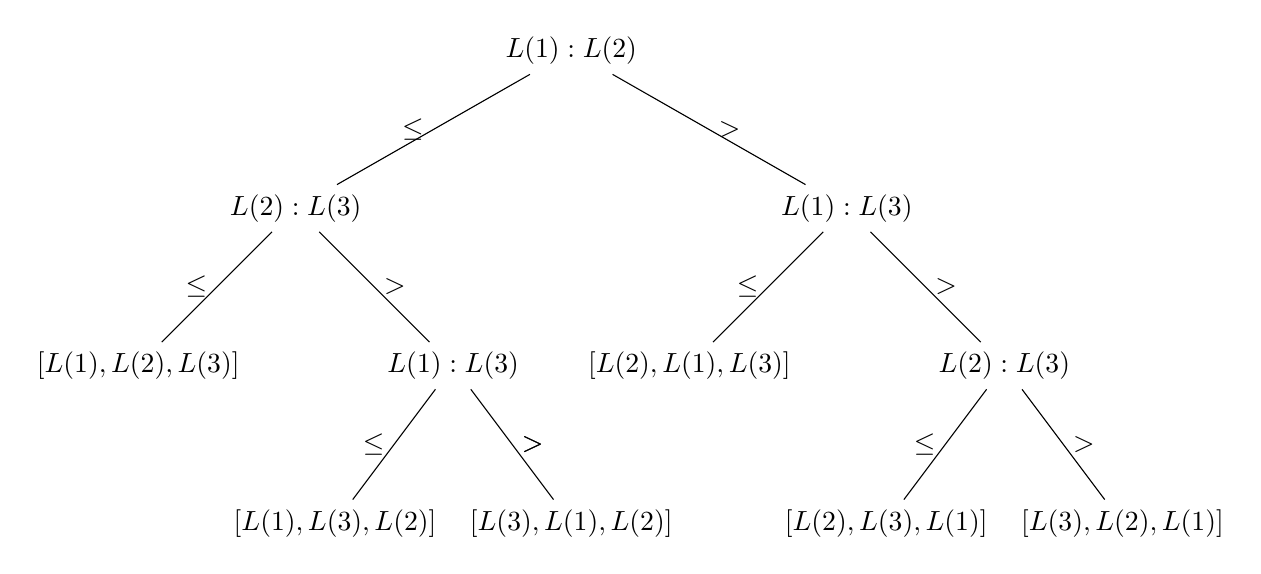
\begin{tikzpicture}[level distance=2cm,
  level 1/.style={sibling distance=7cm},
  level 2/.style={sibling distance=4cm},
  level 3/.style={sibling distance=3cm}]
  \node {$L(1):L(2)$}
    child {node {$L(2):L(3)$} 
      child {node {$[L(1),L(2),L(3)]$} edge from parent node[left]{$\leq$}}
      child {node {$L(1):L(3)$}
          child {node {[$L(1),L(3),L(2)$]} edge from parent node[left]{$\leq$}  }
          child {node {[$L(3),L(1),L(2)$]} edge from parent node[right] {$>$}edge from parent node[right] {$>$}} edge from parent node[right] {$>$}}edge from parent node[left] {$\leq$}
    }
    child {node {$L(1):L(3)$}
    child {node {[$L(2),L(1),L(3)$]}edge from parent node[left]{$\leq$}}
      child {node {$L(2):L(3)$}
      	child {node{$[L(2),L(3),L(1)$]} edge from parent node[left]{$\leq$}   }
      	child {node {$[L(3),L(2),L(1)] $}edge from parent node[right] {$>$}}edge from parent node[right] {$>$}}edge from parent node[right] {$>$}
    };
\end{tikzpicture}
\end{center}

%HACER ÁRBOL CON LO QUE VOY A PONER AHORA MIRA EL SOURCE QUE LO TENGO ESCRITO ORDENAO
%$L(1):L(2)$, si $\leq$, $L(2):L(3)$, si $\leq$ $L(1),L(2),L(3)$
%                                     si $>$ $L(1):L(3)$,        si $\leq$ $L(1),L(3),L(2)$
%                                                                si $>$ $L(3),L(1),L(2)$
%             si $>$, $L(1):L(3)$, si $\leq$ $L(2),L(1),L(3)$ 
%                                     si $>$ $L(2):L(3)$         si $\leq$ $L(2),L(3),L(1)$
%             													SI $>$ $L(3),L(2),L(1)$
\end{ej}

Tenemos la siguiente equivalencia entre propiedades del árbol de decisión y del algoritmo. 
\begin{center}
\begin{tabular}{c|c}
Decision tree & Algoritmo\\
\hline
Nodo & Comparación\\
Hoja & Respuesta\\
Camino Raíz-Hoja & Ejecución\\
Longitud camino R-H & Running time\\
Altura & Máximo tiempo de ejecución
\end{tabular}
\end{center}

Denotamos $h$ a la altura del árbol y $l$ al número de hojas. Es claro que $l\leq 2^h$, y como las hojas nos dan permutaciones de la lista, $l\geq n!$. De aquí deducimos que $2^h\geq n!$, de donde 
$$h\geq \log n!=\sum_{i=1}^n\log i\geq \sum_{i=\frac{n}{2}}^n\log i\geq \sum_{i=\frac{n}{2}}^n\log\left(\frac{n}{2}\right)=\sum_{i=\frac{n}{2}}^n(\log n-1)=\frac{n}{2}\log n-\frac{n}{2}\in\Omega(n\log n)$$
Esto prueba el teorema. 
\end{document}
